\documentstyle[cec2003,multicol,times,epsfig]{article}

\begin{document}
\pagestyle{empty}
\sloppy

\twocolumn[
\title{SimME\\Mobile Multiplayer Gaming}

\vspace{2mm}
\begin{multicols}{4}
\begin{center}
	Wolfgang Slany\\
	\emph{Project Lead}\\
	wsi@ist.tugraz.at
\end{center}
\begin{center}
	Paul Sprenger\\
	\emph{Technical Documentation}\\
	sprenger@sbox.tugraz.at
\end{center}
\begin{center}
	Georg Spielmann\\
	\emph{User Interface}\\
	shurli@users.berlios.de
\end{center}
\begin{center}
	Kariem Hussein\\
	\emph{Architecture and Design}\\
	kariem@users.berlios.de
\end{center}
\end{multicols}
\vspace{0.25in}
] % end of the argument to \twocolumn

\begin{abstract}

	SimME is a multiplayer game for mobile devices (mobile phones, PDAs, ...)
	developed to provide a basis for a gaming forum in which new games can
	easily be integrated. The architecture described in this document is
	targeted on assisting the implementation of multiplayer games for mobile
	devices.

\end{abstract}

\section{Introduction}

	A lot of game developers, particulary developers working in the area of
	wireless communication, are confronted with the same problem: a two player
	game is usually limited to infrared or bluetooth communication, depending on
	the device capabilities. A server-based version for multiplayer gaming is
	unlikely, due to limited resources on mobile devices.

	On the basis of this consideration the SimME project tries to create a
	platform in which a server-based multiplayer version of an existing game can
	be created with minimal effort. The communication is based on internet
	technologies, a domain where most mobile device vendors focus their
	development.

	Because of the strict partitioning of game logic and communication between
	client and server, we have achieved that the server-side only has to
	implement the communication protocol between client and server. In fact, the
	server is only a mean of documented communication. Games could be viewed at
	a later point in time and player performance can be logged and compared.

	\subsection{Description of the game SimME}

		SimME is a game based on the Ramsey-theorem, describing the party
		puzzle, a special case of the Ramsey theory. The game board consists of
		six points arranged in an hexagon, each of which is linked to the other
		five points. At each turn, one player connects two points. The player
		who connects three points with a triangle loses the game. Figure
		\ref{fig:gameboard} shows how the application looks on the client
		device.

		\begin{figure}[h]
		\begin{center}
			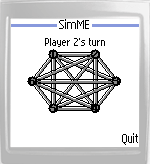
\includegraphics{pics/simme-screen.png}
			\caption{SimME game board on mobile phone}
			\label{fig:gameboard}
		\end{center}
		\end{figure}

		The game can never end in a draw, there is always a winner. Due to the
		odd number of connections between the vertices of the hexagon, there can
		never be a stalemate. A close analysis of this game and the underlying
		Ramsey theory was done in the paper \emph{Graph Ramsey games} by
		Wolfgang Slany \cite{slany_paper}.

		The game is designed for mobile phones and allows either to play against
		the computer, or against another human player over the web. Therefor the
		game has a client-server architecture. More on this in section
		\ref{sec:architecture}.


\section{Current State of Development}

	Until now the game SimME was implemented in the following versions:

	\noindent as \emph{one player game (against a computer opponent)}, as
	\emph{local multiplayer game (two players - one device)} and as
	\textit{multiplayer game (with an external game server)}.

	The main focus lied on the strict isolation of client and server, to design
	game logic and communication between client and server as modular as possible,
	for a good reusability for other games.
	
	A close look on the architecture follows in section \ref{sec:architecture}.
	
	\begin{enumerate}
	
		\item \textit{one player game (against a computer opponent)}
		
			A computer opponent is implemented. As described in section
			\ref{sec:ci} at this time there is no \textit{intelligent} computer
			opponent integrated in the game SimME, but an opponent taking
			randomised turns.
			
			The portation of a learning computer opponent, implemented as a
			Java-Applet Version of the game (called HEXI) from Univ.-Prof.
			Dipl.-Ing. Dr.techn. Wolfgang Slany, is planned \cite{slany_paper}.
			
		\item \textit{local multiplayer game (two players - one device)}
		
			In this Version of the game SimME two players play local against
			each other. They share one mobile device an take turns one after the
			other.
			
			A local multiplayer game Version will be the starting point
			for implementing a server based version of other games in the
			future.
			
		\item \textit{multiplayer game (with an external game server)}
		
			This Version of the game is using the design described in section
			\ref{sec:architecture}. Two human players are connecting to a game
			server, using their mobile device, which controls the communication
			between the two players and checks the data content.
			
	\end{enumerate}
	
	With these three game layouts the porting of an existing game to the
	SimME-platform can be described.


\section{Going online} \label{sec:going_online}

	\begin{figure*}[htbp]
		\begin{center}
			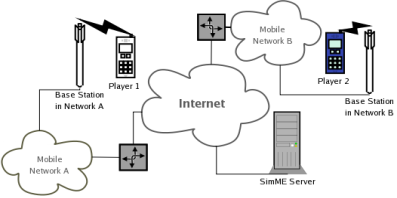
\includegraphics{pics/communication-small.png}
			\caption{Communication between clients on two different networks}
			\label{fig:communication}
		\end{center}
	\end{figure*}

	Starting from a game - a local multiplayer game (Point 1 and 2 of the Present
	Development State) - it's easy to implement the communikation between two
	clients using an external server.
	
	The task is to create an interface used by the server and the client to
	communicate with each other.
	
	In which way can this interface be built? The SimME-server provides some base
	classes, supporting the communication for 2 player-games. Using the protocol,
	given by the SimME-server, the realisation of a serverbased multiplayer version
	of a game is no problem any longer.
	
	At the client side of the game there are just a few modifications to realise.
	An interface has to be implemented which has to wait for turns, sent by the
	game server. Besides this no other changes have to be done, no alterations in
	the game logic or the game-flow have to be done.

	\begin{figure}[h]
	\begin{center}
	%\epsfig{file=./pics/internal_interface.png, scale=0.6}
	\caption{Internal Interface}
	\end{center}
	\end{figure}


\section{Design and Architecture} \label{sec:architecture}

	As already said in section \ref{sec:going_online}, the game server can be
	seen as sole mediator between the game clients. The server has no access to
	the game logic, though it uses the client classes to verify correct
	gameplay.

	\subsection{Advantages of the separation of server and game logic}

		Because of the separation of the game logic from the server, the server
		is nothing more than a link between the two players. All game internal
		check-ups are done by the clients and so the server is not charged.
		
		Further on its guaranteed that no \textit{needless information} is
		transferred. For example an illegal game turn is not transferred to the
		server, because the validation of moves is done in the clients. So the
		illegal turn will never arrive at the server or the second player.

	\subsection{Communication between client and server}

		The communication between client and server uses two different types of
		communication. On the one hand the client sends direct HTTP-requests, on
		the other hand the server answers with XML content. Figure
		\ref{fig:com_client_server} illustrates this.

		\begin{figure}[h]
		\begin{center}
			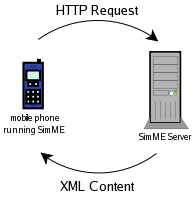
\includegraphics{pics/com_client_server.png}
			\caption{Communication between client and server}
			\label{fig:com_client_server}
		\end{center}
		\end{figure}

		The communication interface is backed by dynamic menus, created and
		administrated by the game server. These dynamic menus can be reused by
		other games because they are organised in interface-classes and
		consequently are modular. The layout and content is defined in XML and
		can be exchanged at run-time.

	\subsection{Internal administration on the server}
	
		The internal data organisation on the server side is carried out by
		means of a database, containing informations about the games currently
		running and about registered players. Further on with this database also
		the different games, implemented on the SimME-platform, will be
		administrated.
		
		Thus information about currently registered players, running games, and
		so on can be obtained via SQL statements.
		
		One of our next goals is to implement, alternatively to improve, the
		statistic part of the database. In this way statistics about gaming
		behaviour, win-lose statistics and much more can be implemented.


\section{Computational Intelligence} \label{sec:ci}

	At the current state of development there is no implementation of a CI
	gaming unit available on the SimME-server. The same game (also known under
	the name of HEXI) was realised as a java applet by Wolfgang Slany. In this
	version of the game, playable on
	\textit{http://www.dbai.tuwien.ac.at/proj/ramsey/} a learning computer
	opponent is implemented. You can take a closer look on the implementation of
	this CI gaming unit in \cite{slany_paper}
	
	\noindent Online version of this paper:\\
	http://www.dbai.tuwien.ac.at/ftp/papers/slany/dbai-tr-99-34.ps.gz

	\subsection{CI Player for SimME}
	
		The CI gaming unit mentioned above will be integrated in the single
		player version of the game SimME. On the client as on the server side.
		Through the implementation of the CI gaming unit on the SimME-server we
		get the possibility to record statistics about gaming strategies,
		because sole moves and therefor whole game matches could be logically
		analysed.
		
		Furtheron the learning CI gaming unit could even \textit{learn} from
		matches played by two human players.
		
		Based on these statistics an adjustment of gaming levels of the
		CI-gaming-unit could be done, so to each player a CI player with the
		same gaming level can be assigned.


\section{Look-out on future developments}

	In this section some ideas are listed we will implement in the future.
	
	\subsection{Communication betwen the players during a running game}
	
		Like Tony Manninnen says in "Interaction Forms and Communicative Actions
		in Multiplayer Games" \cite{mann03}:
		
		\begin{quotation}
		
			Rich interaction is achieved through direct manipulation of objects,
			multimodal input devices and the high number of degrees of freedom.
			However, this relatively technical definition covers only one
			portion of the concept. In addition to these, social, cultural and
			communicative aspects have a significant impact on interaction
			richness. [...]
		
			\textit{Rich interaction does not necessarily require rich
			interfaces.}
			
		\end{quotation}
		
		The last sentence of this quotation describes our approach to useful
		communication forms between players really good. The idea is to provide
		some \emph{hardcoded} sentences which can be sent to the second player.
		In the first place its a very time saving way to communicate in written
		form - which is important because of the online costs of mobile devices.
		Secondly, with fixed sentences, a database can be used for translating
		these sentences to different languages at minimal costs.
		
		Of course it is also planned to implement a chat functionality to aid a
		free form of communication.
	
	\subsection{Integration of the CI gaming unit at the client and the server}

		As described in \ref{sec:ci} a CI gaming unit will be integrated in the
		SimME server and on client side, to support a challenging single player
		version one the one hand, and to improve the value of game statistics on
		the other hand.
		
		The CI gaming unit implemented by Wolfgang Slany is a learning opponent,
		so the recorded games will be used by the CI gaming unit to improve the
		playing style.
	
	\subsection{Improved game statistics}


\newpage

\begin{thebibliography}{10}

	\bibitem[slany99]{slany_paper} Slany W. (1999) "Graph Ramsey games",
	Institut f\"{u}r Informationssysteme Abteilung Datenbanken und Artificial
	Intelligence Technische Universit\"{a}t Wien
	
	\bibitem[mann03]{mann03} Manninen T. (2003) "Interaction Forms and
	Communicative Actions in Multiplayer Games", The international journal of
	computer game research
	
\end{thebibliography}

\end{document}
